\documentclass[a4paper,12pt]{article}
\pdfpagewidth
\paperwidth
\pdfpageheight
\paperheight
\usepackage[english]{babel}
\usepackage[utf8]{inputenc}
\usepackage[babel]{csquotes}    %per biblatex
\usepackage{biblatex}   %bibliografia
% \usepackage{xurl}  %per mandare a capo gli url in bibliografia
%\setcounter{biburllcpenalty}{7000}  %per mandare a capo gli url in bibliografia
%\setcounter{biburlucpenalty}{8000}  %per mandare a capo gli url in bibliografia
%\def\UrlBreaks{\do\/\do-}
\usepackage{epsfig}
\usepackage{fancyhdr} 
\usepackage{amsmath,amssymb}
\usepackage{amscd} 
\usepackage[T1]{fontenc} 
\usepackage[usenames,dvipsnames]{xcolor}
\usepackage{graphicx,color,listings}
\graphicspath{{img/}}
%\usepackage{array}
\usepackage{placeins}   %per \floatbarrier
\usepackage{hologo}
\frenchspacing
\usepackage{rotating}
\usepackage[bf,small]{caption}
\captionsetup{tableposition=top,figureposition=bottom,font=small}
\usepackage{textcomp, gensymb}  %textcomp è per usare % e altri simboli
\usepackage{hyperref}
\hypersetup{colorlinks=true, linkcolor=black, filecolor=blue, urlcolor=blue}
\usepackage{multirow}
\usepackage{picture}
\usepackage{booktabs}
\usepackage{subfig}
\usepackage{float}  %per [H]
%\usepackage{circuitikz}    %circuiti
\usepackage[separate-uncertainty=true]{siunitx} %unità di misura
\usepackage{newlfont}
\textwidth=450pt\oddsidemargin=0pt
\usepackage{setspace}   %interlinee diverse
\usepackage[version=4]{mhchem}  %formule chimiche

\bibliography{bib}

\title{BCM model as images generator}
\author{Tommaso Rondini}

\begin{document}
\maketitle

\section{Introduction}
The BCM model is a neural network which is able to classify images in clusters given training data without labels (so it learns in unsupervised way).
Looking to the neurons' weights after the training step they could be mapped into an image similar to the training ones.
The ``neuron's weights'' are the importance that the neuron gives to each pixel to classify the images, so how much the intensity of that pixel is relevant to recognise if the image belongs to the cluster or not.
Obviously the weights are expressed by numbers and not by images, but they can be mapped to obtain a grey scale image.
This concept can be applied to colour images too, using the weights of each channel as colour intensity in the synthetic image.
In this report I use only grey scale images.

\subsection{BCM model}
The BCM model was inspired by a study of neurons in the visual cortex  conducted by Elie Bienenstock, Leon Cooper, and Paul Munro in 1982\cite{BCM:1982}.
In the following years it underwent changes; I use the model proposed by Law and Cooper in 1994\cite{law:1994} and then adapted adding lateral connections thanks to the contribution of Castellani et al.\cite{castellani:1998}.
In biology, lateral connections are synaptic links between neurons inside visual cortex.
The connections can be positive (if a neuron recognizes a cluster of data, it suggests others to recognize the same type) or negative (it suggests  others to find other weights so that they will find different clusters).
In the BCM model a matrix is used to express these relationships and we call it \emph{interaction matrix}\cite{cooper:1988}.
I use two matrices in this project:
\begin{itemize}
\item[\emph{L}] a matrix where all the elements are equal so it creates only negative connections;
\item[\emph{B}] a matrix that creates negative connections between all neurons except between couples.
\end{itemize}
The matrix \emph{B} has a biological justification: in our brain the visual cortex is split in two hemispheres, the left and the right.
Simplifying we can say that the information acquired by the left eye arrives to the right hemisphere and vice versa.
But the eyes receive more or less the same information (except for a different angle and the peripheral vision), so both the hemispheres recognise the same object.
The \emph{B} matrix reproduces this behaviour\cite{berselli:2023}.
An example of \emph{B} matrix is given in Eq.\ref{eq:matrixB}.
\begin{equation}\label{eq:matrixB}
  \begin{bmatrix}
    1. &  0.2 & -0.3 & 0.2 & -0.3 \\
    0.2 & 1. & -0.3 & -0.3 & 0.2 \\
    -0.3 & -0.3 & 2.3 & -0.3 & -0.3 \\
    0.2 & -0.3 & -0.3 & 1. & 0.2 \\
    -0.3 & 0.2 & -0.3 & 0.2 & 1.
  \end{bmatrix}
\end{equation}

\subsection{Synthetic images estimation}
Once the synthetic images are created, we need to evaluate their quality in order to understood which combination of parameters reproduces the best results.
First of all, a qualitative opinion is attended, simply looking the pictures.
However, a quantitative judgement is necessary: I use the \emph{Fréchet Inception Distance} (FID)\cite{heusel:2017}, commonly used to evaluate synthetic images generated by \emph{Generative Adversarial Networks} (GANs).
It calculates the distance between the training images distribution and the synthetic images one.
I try to use other methods, such as the \emph{Peak Signal to Noise Ratio} (PSNR) and the \emph{Structural SIMilarity} (SSIM), but they are generally used to compare two pictures at time and I have to manage datasets.
I calculate the \emph{Precision, Recall, Density and Coverage} (PRDC)\cite{naeem:2020}, but they produce results discordant with visual and FID judgements.

\subsection{Compilation info}
The elements' values of the interaction matrices are copied by above articles, so $L$ has a negative connection value $-0.5$, while $B$ has as negative connection $-0.2$ and as positive $0.3$.
The implementation of the BCM model is the \emph{Python} version of Curti et al.\cite{curti:2020} with a few adjustments in order to make faster the graphical representation of results.
The training dataset is the Olivetti faces, that is a collection of ten pictures of forty people's faces in grey scale, $8$bit and $64 \times 64$ size.
To evaluate the FID I use a \emph{Pytorch} module\cite{seitzer:2020}.
Each model is trained for $3000$ epochs.
The $B$ matrix generates a synthetic ``average'' image of all the training images, while all the other neurons highlight the differences of the clusters which they select.
Instead, the $L$ matrix generates a synthetic image for each neuron.
In consequence, the $B$ matrix creates only one image for training, meanwhile the $L$ creates as many images as the number of neurons ($N$).
When the batch size is not specified it is $10$.
The FID's calculation requires a distribution with that to compare the synthetic images' one.
I use the distribution of the all Olivetti dataset; in this way I can compare all the FIDs between them.


\section{Comparison between matrices}
As first study I check which matrix produces better images, so that other studies will be attended with it.
For each matrix I attend two types of simulation: one using as dataset faces of the same person, the other using faces of different people.
With the same dataset I change the number of neurons of the model: \numlist{5;9;13;17;21}.
I repeat the same type of simulation five times, changing the dataset but not its features.
Since for each person I have ten pictures, the datasets are composed by ten images for all the simulations.
For each model with each dataset I save $64$ synthetic images, changing the weights initialization.

In Fig.\ref{fig:greg_curti_g} we see the FID depending on $N$.
I change a little the x axis' values since improve visualization, but all the simulations are done with the same (and integer) number of neurons.
We see that for a few neurons the better results are achieved by simulation with faces of the same person.
Increasing $N$, the type of matrix is more significant: the $B$ matrix achieves better results for the same number of neurons.
The same observations can be done looking the synthetic pictures.
In Fig.\ref{fig:greg_curti_p} some of the synthetic images of the simulations are showed.
Since these result, future simulations are attended with $B$ matrix.

\begin{figure}[!hbt]
  \centering
  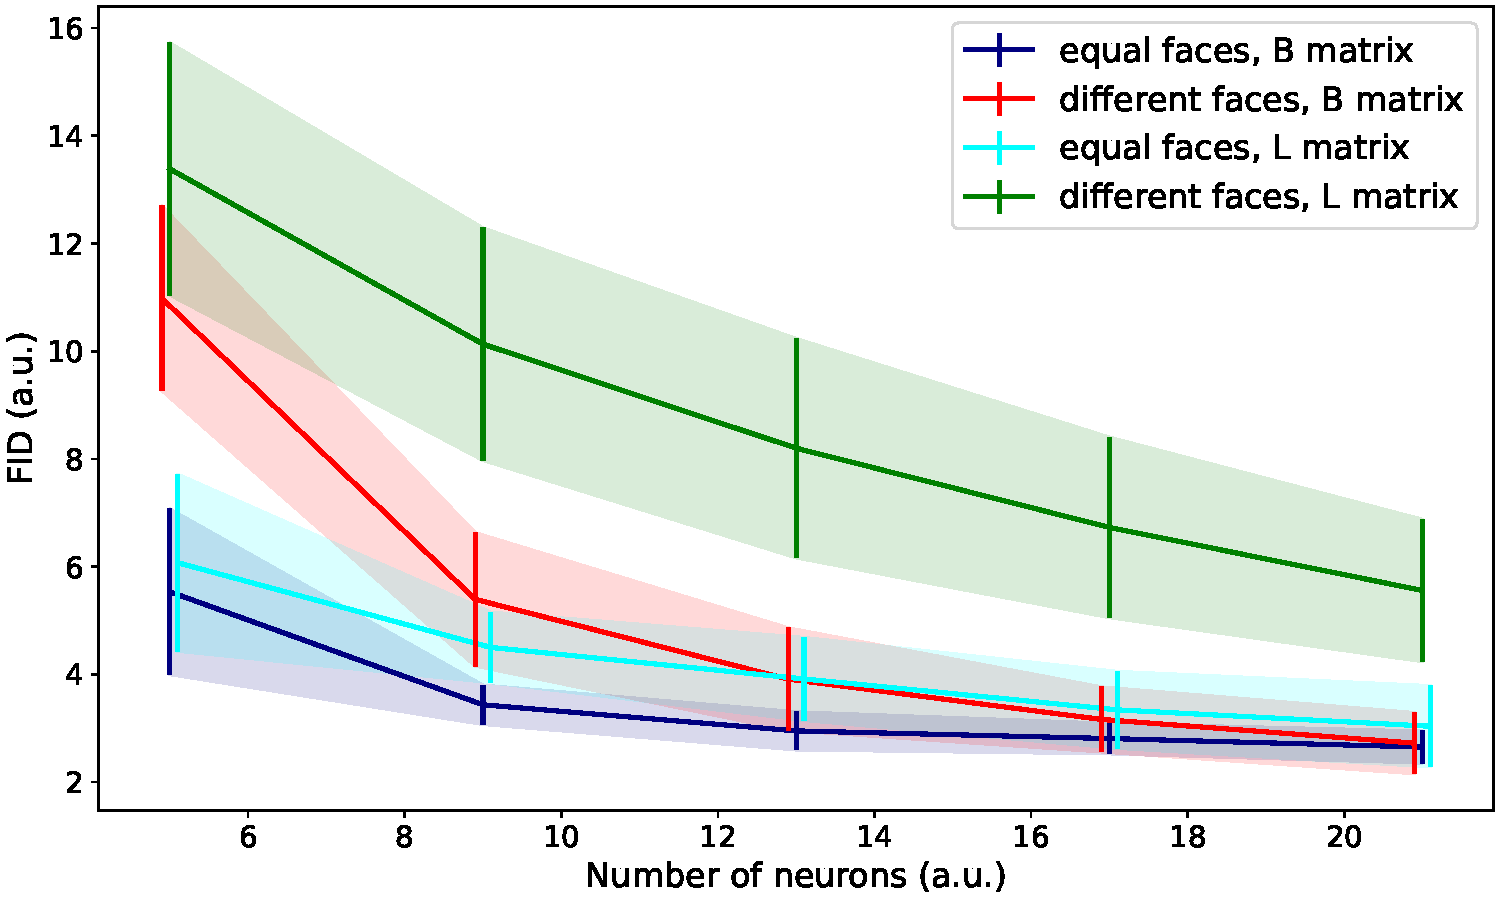
\includegraphics[width=.9\columnwidth]{greg_curti.pdf}
  \caption[FID of $L$ versus $B$ matrix]{The evolution of the FID in relation to Olivetti dataset depending on the number of neurons.
  Two simulations are made with $L$ matrix and two with $B$ matrix; one with the pictures of the same person, the other with random faces.
  Each simulation is repeated five times and the error bars are the standard deviation of the FID in each case.
  Each dataset is made up ten pictures.
  }
  \label{fig:greg_curti_g}
\end{figure}

\begin{figure}[!htbp]
  \centering
  \subfloat[][\emph{5 N, B, same faces}]{
    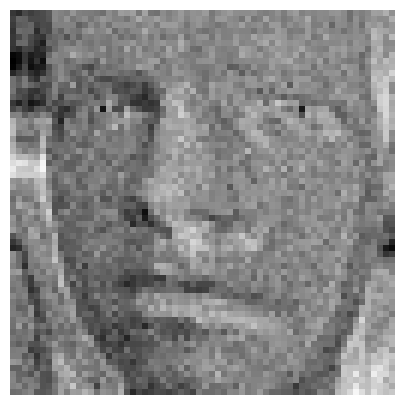
\includegraphics[width=.24\columnwidth]{a}} 
  \subfloat[][\emph{5 N, B, diff. faces}]{
    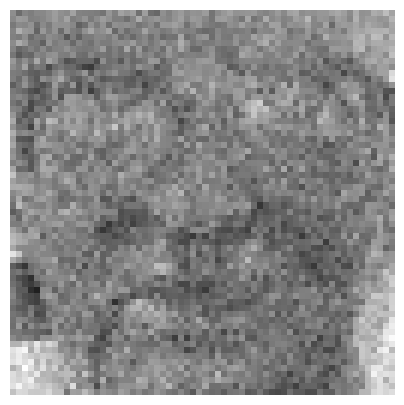
\includegraphics[width=.24\columnwidth]{b}}
  \subfloat[][\emph{5 N, L, same faces}]{
    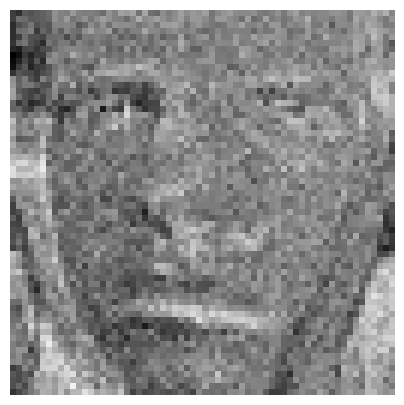
\includegraphics[width=.24\columnwidth]{c}} 
  \subfloat[][\emph{5 N, L, diff. faces}]{
    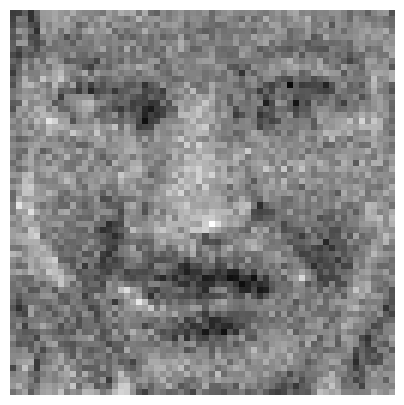
\includegraphics[width=.24\columnwidth]{d}}\\
  \subfloat[][\emph{21 N, B, same faces}]{
    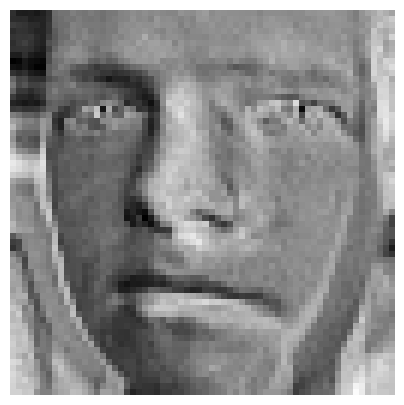
\includegraphics[width=.24\columnwidth]{e}} 
  \subfloat[][\emph{21 N, B, diff. faces}]{
    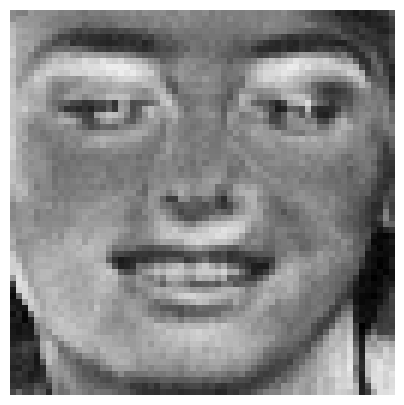
\includegraphics[width=.24\columnwidth]{f}}
  \subfloat[][\emph{21 N, L, same faces}]{
    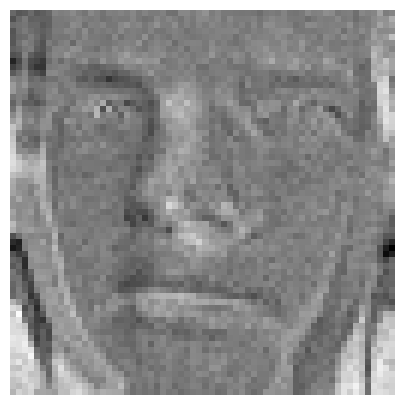
\includegraphics[width=.24\columnwidth]{g}} 
  \subfloat[][\emph{21 N, L, diff. faces}]{
    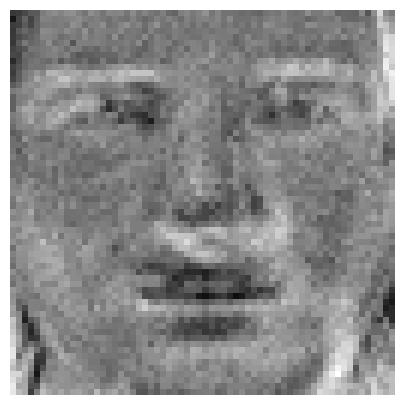
\includegraphics[width=.24\columnwidth]{h}}
  \caption[Picture of $B$ versus $L$ matrix]{One synthetic picture for each type of simulation with $5$ and $21$ neurons.
  The first four are synthetic images generated with $5$ neurons with different matrices and datasets.
  Below each of them there is the synthetic image with the same matrix and data but generated with $21$ neurons.}
  \label{fig:greg_curti_p}
\end{figure}

\section{Comparison between dataset size}
Beyond the two previous simulations with $B$, I change the dataset size to see which gives better results.
Also for these simulations I repeat them five times and generate $64$ images changing initial weights.
The number of neurons are still \numlist{5;9;13;17;21}.
The studied cases are:
\begin{itemize}
  \item $5$ pictures of the same person;
  \item $5$ random pictures;
  \item $10$ pictures of the same person (above simulation);
  \item $10$ random pictures (above simulation);
  \item $20$ pictures of the same two people;
  \item $20$ random pictures.
\end{itemize}
The case of $20$ pictures of two people is a bit different from the others since it mixs two people.
I do it because I need to increase the dataset size and I have at the maximum $10$.
In the cases with $5$ picture as dataset, the batch's size is $5$.

In Fig.\ref{fig:greg_g} we see that increasing $N$ the FID seems to converge, but for a few neurons the behaviour is totally different.
With an high $N$, we notice that the larger datasets have a better FID than smaller ones.
The same thing happens for datasets of the same person respect to random datasets.
The datasets made of $20$ pictures achieve the best FID (with great $N$) of all.
We notice that the random dataset is better than the one made up two people's faces.

In Fig.\ref{fig:greg_p} I quote one synthetic image for simulation, always generated with $21$ neurons.
Qualitatively we can not see great differences between them, except the synthetic image generated with $5$ pictures of the same person (Fig.\ref{fig:greg_p_5same}), that is the worst.
It is a confirmation that the FID is a good estimation of the visual evaluation, since in Fig.\ref{fig:greg_g} we see that the worst FID at $21$ neurons is just with the $5$ same person pictures dataset and all the other are more similar one each others.

\begin{figure}[!htbp]
  \centering
  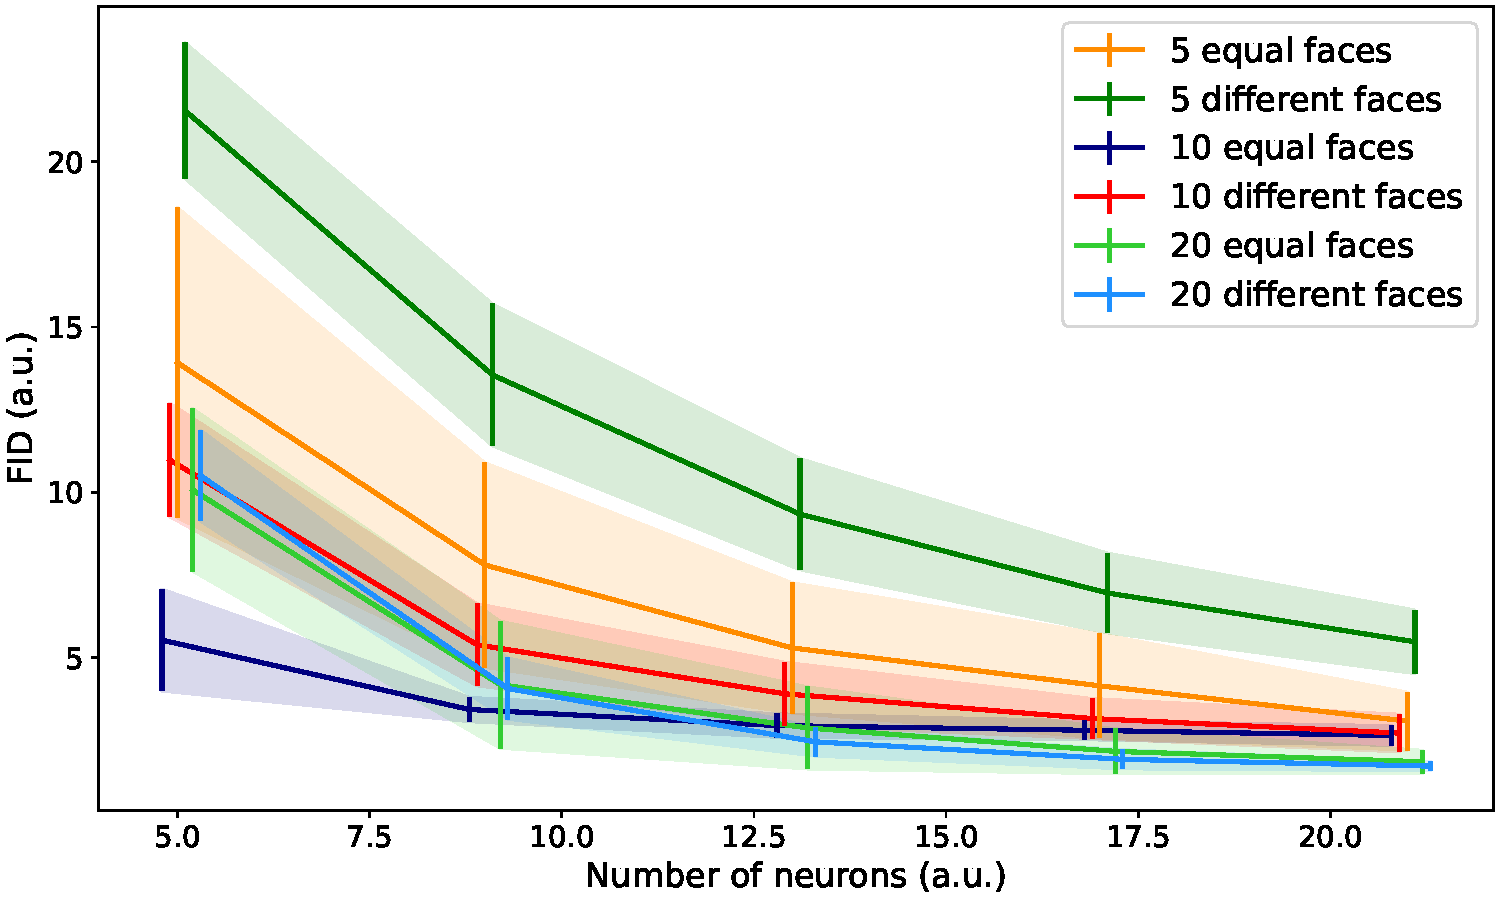
\includegraphics[width=.9\columnwidth]{greg.pdf}
  \caption[FID changing dataset size]{The evolution of the FID in relation to Olivetti dataset depending on the number of neurons.
  For the same dataset size (\numlist{5;10;20}) there are two simulation: one with pictures of the same person; the other with random pictures.
  Each simulation is repeated five times and the error bars are the standard deviation of the FID in each case.
  The interaction matrix is always $B$.
  }
  \label{fig:greg_g}
\end{figure}

\begin{figure}[p]
  \centering
  \subfloat[][\emph{size 5, same faces}]{
    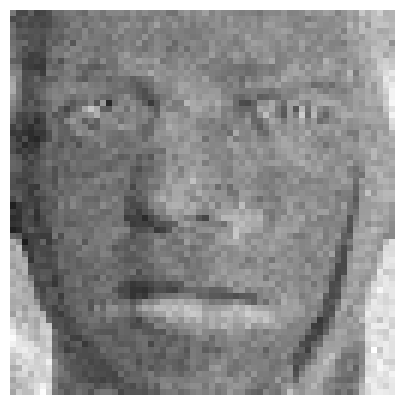
\includegraphics[width=.3\columnwidth]{i}
    \label{fig:greg_p_5same}}
  \subfloat[][\emph{size 5, diff. faces}]{
    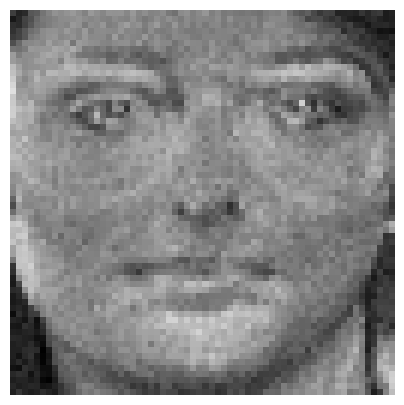
\includegraphics[width=.3\columnwidth]{l}} \\
  \subfloat[][\emph{size 10, same faces}]{
    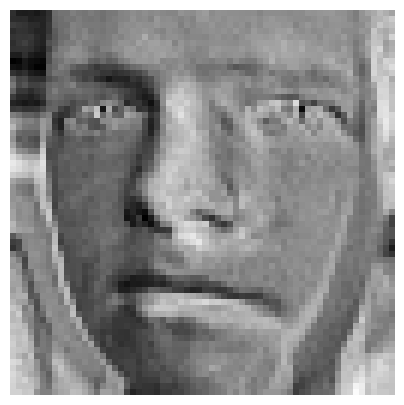
\includegraphics[width=.3\columnwidth]{e}}% \quote
  \subfloat[][\emph{size 10, diff. faces}]{
    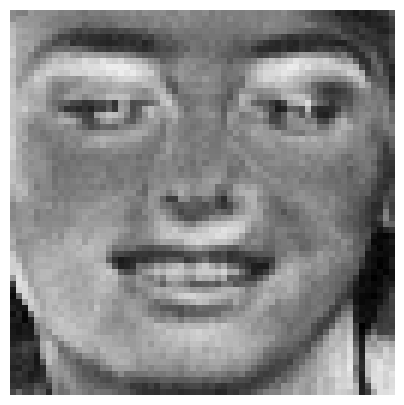
\includegraphics[width=.3\columnwidth]{f}}\\
  \subfloat[][\emph{size 20, same faces}]{
    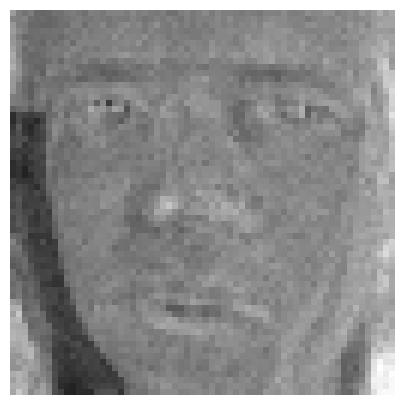
\includegraphics[width=.3\columnwidth]{m}}% \quote
  \subfloat[][\emph{size 20, diff. faces}]{
    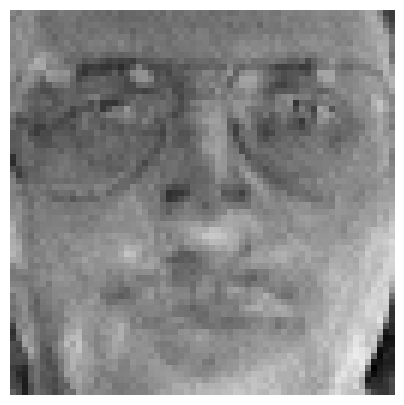
\includegraphics[width=.3\columnwidth]{n}}
  \caption[Picture with different dataset's size]{One synthetic picture for each dataset type.
  In the first column there are the picture generated with datasets made up same people's faces; in the second with datasets made up random faces.
  For each row, the dataset size is the same, so in the \numlist{1;2;3} row there are pictures with dataset size of \numlist{5;10;20} respectively.
  The number of neurons is always $21$.
  }
  \label{fig:greg_p}
\end{figure}

\section{Comparison between batch size}
Since in above section we see that the best FID is achieved by a dataset of $20$ random faces, I decide to use as training dataset all the Olivetti's pictures.
Then, I increase the number of neurons of the model (since better results are attended with high $N$) and I try with \numlist{21;25;29}.

The last parameter to test is the batch size.
Until now it was almost always $10$; now I select \numlist{10;20;50;100}.
Since I use the whole dataset, I can not reply the simulations five times, so in Fig.\ref{fig:all_g} there is not the standard deviation of the FID.

The FID's trend does not highlight any common features or a more efficient batch.
The two best results have batch $100$ and $N$ respectively equal to \numlist{21;29}, but with $N$ equal to $25$ the FID has a spike.
On the contrary, the FID with batch $20$ has a minimum with $N$ equal to $25$.
With batch of  \numlist{10;50} FIDs are monotonic: the first is decreasing, the second is increasing.

The synthetic images generated with the smallest FID (batch equal to $100$ and $N$ equal to $21$) are qualitative good, too, as you can see in Fig.\ref{fig:all_p}.
Unfortunately, using all the dataset most of them are very similar and, between $64$ generated, there are only three different faces.

\begin{figure}[!htb]
  \centering
  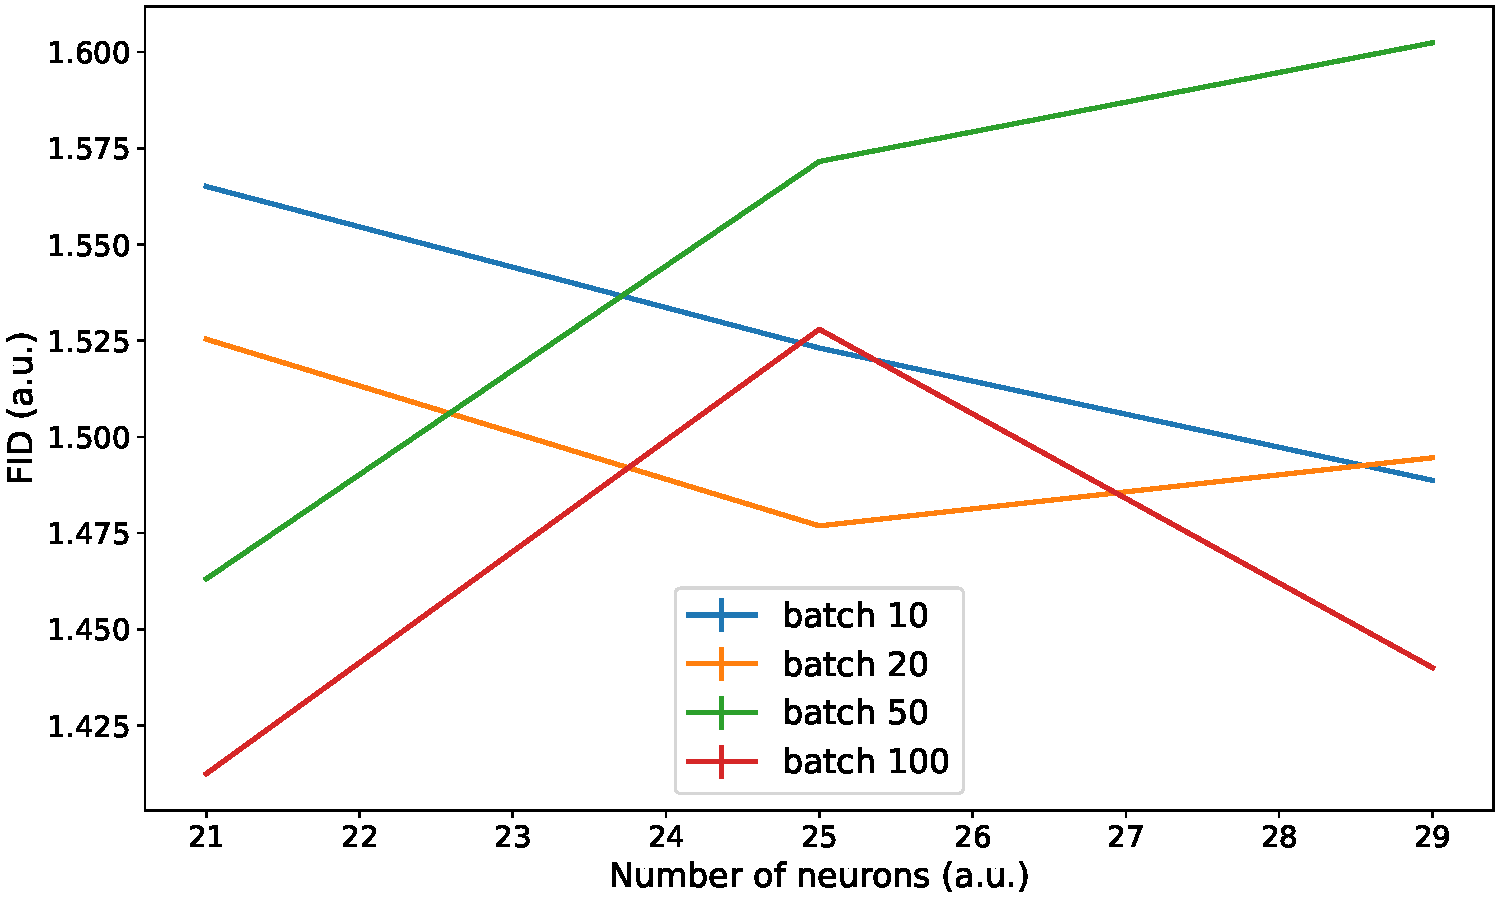
\includegraphics[width=.9\columnwidth]{all.pdf}
  \caption[FID changing batch's size]{The evolution of the FID in relation to Olivetti dataset depending on the number of neurons.
  There is used always all the dataset, but the batch size changes.
  The interaction matrix is always $B$.
  }
  \label{fig:all_g}
\end{figure}

\begin{figure}[!htb]
  \centering
  \subfloat[][\emph{56 occurences}]{
    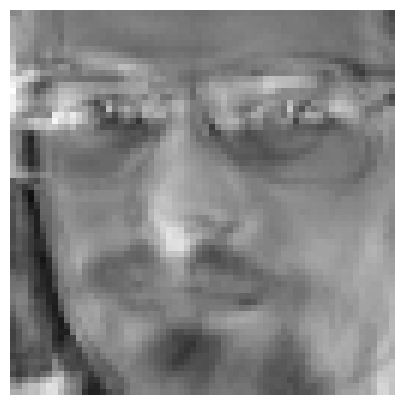
\includegraphics[width=.3\columnwidth]{o}}
  \subfloat[][\emph{7 occurences}]{
    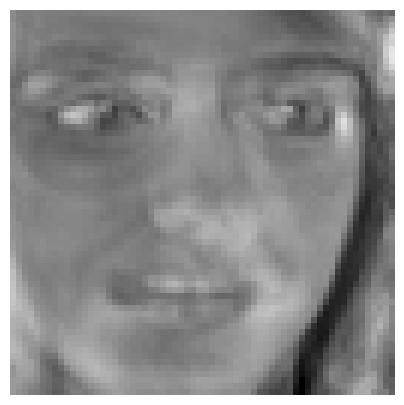
\includegraphics[width=.3\columnwidth]{p}}
  \subfloat[][\emph{1 occurence}]{
    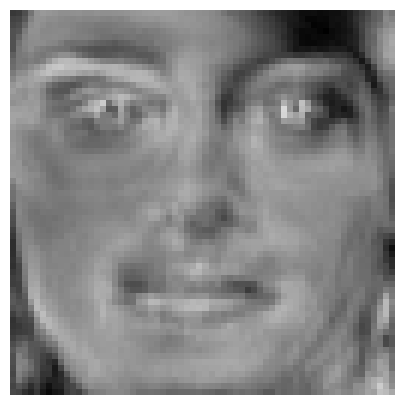
\includegraphics[width=.3\columnwidth]{q}}
  \caption[Pictures with batch $100$ and $N$ $21$]{Three synthetic pictures with batch size equal to $100$ generated by a BCM model with $21$ neurons and interaction matrix of type $B$.
  All the other generated images ($61$) are similar to these three.
  The occurrence of each example is reported in its sub-caption.
  }
  \label{fig:all_p}
\end{figure}

\section{Conclusions}
Given a dataset, to generate synthetic images throw a BCM model is on the whole possible.
You get images resembling those of training mapping neurons' weights.
Modifying the parameters and the dataset you achieve quite good images: the better combination of them that I found is with $21$ neurons, interaction matrix of type $B$ and batch's size equal to $100$, using as training dataset the whole Olivetti.
The FID of this simulation is $1.412$.

However the synthetic pictures are neither qualitatively nor quantitatively indistinguishable from the training ones.
I am not able to determine any rules to find the best results, since increasing $N$ does not always reduce FID either (see Fig.\ref{fig:all_g}).
I can say that the matrix $B$ returns better results, but generates less images.

Ultimately, if on the whole the model can be used to synthesize images, at the state of the art it can not generate qualitatively indistinguishable images from real ones, much less to compete with others existing synthesizers.
Furthermore, the latter can generate hypothetically infinite images once they are trained; on the contrary the BCM model needs to be trained for each synthetic image.

\clearpage
\addcontentsline{toc}{section}{\refname}
\printbibliography
\end{document}
